
\begin{figure}[p]

    \noindent\makebox[\textwidth]{
        \centering
        %\includegraphics[width=0.8\textwidth]{../../sympy/catalan/coloured.pdf}

        % using *angle* property to rotate it is difficult to properly align it
        % in order to have a "real" matrix representation.
        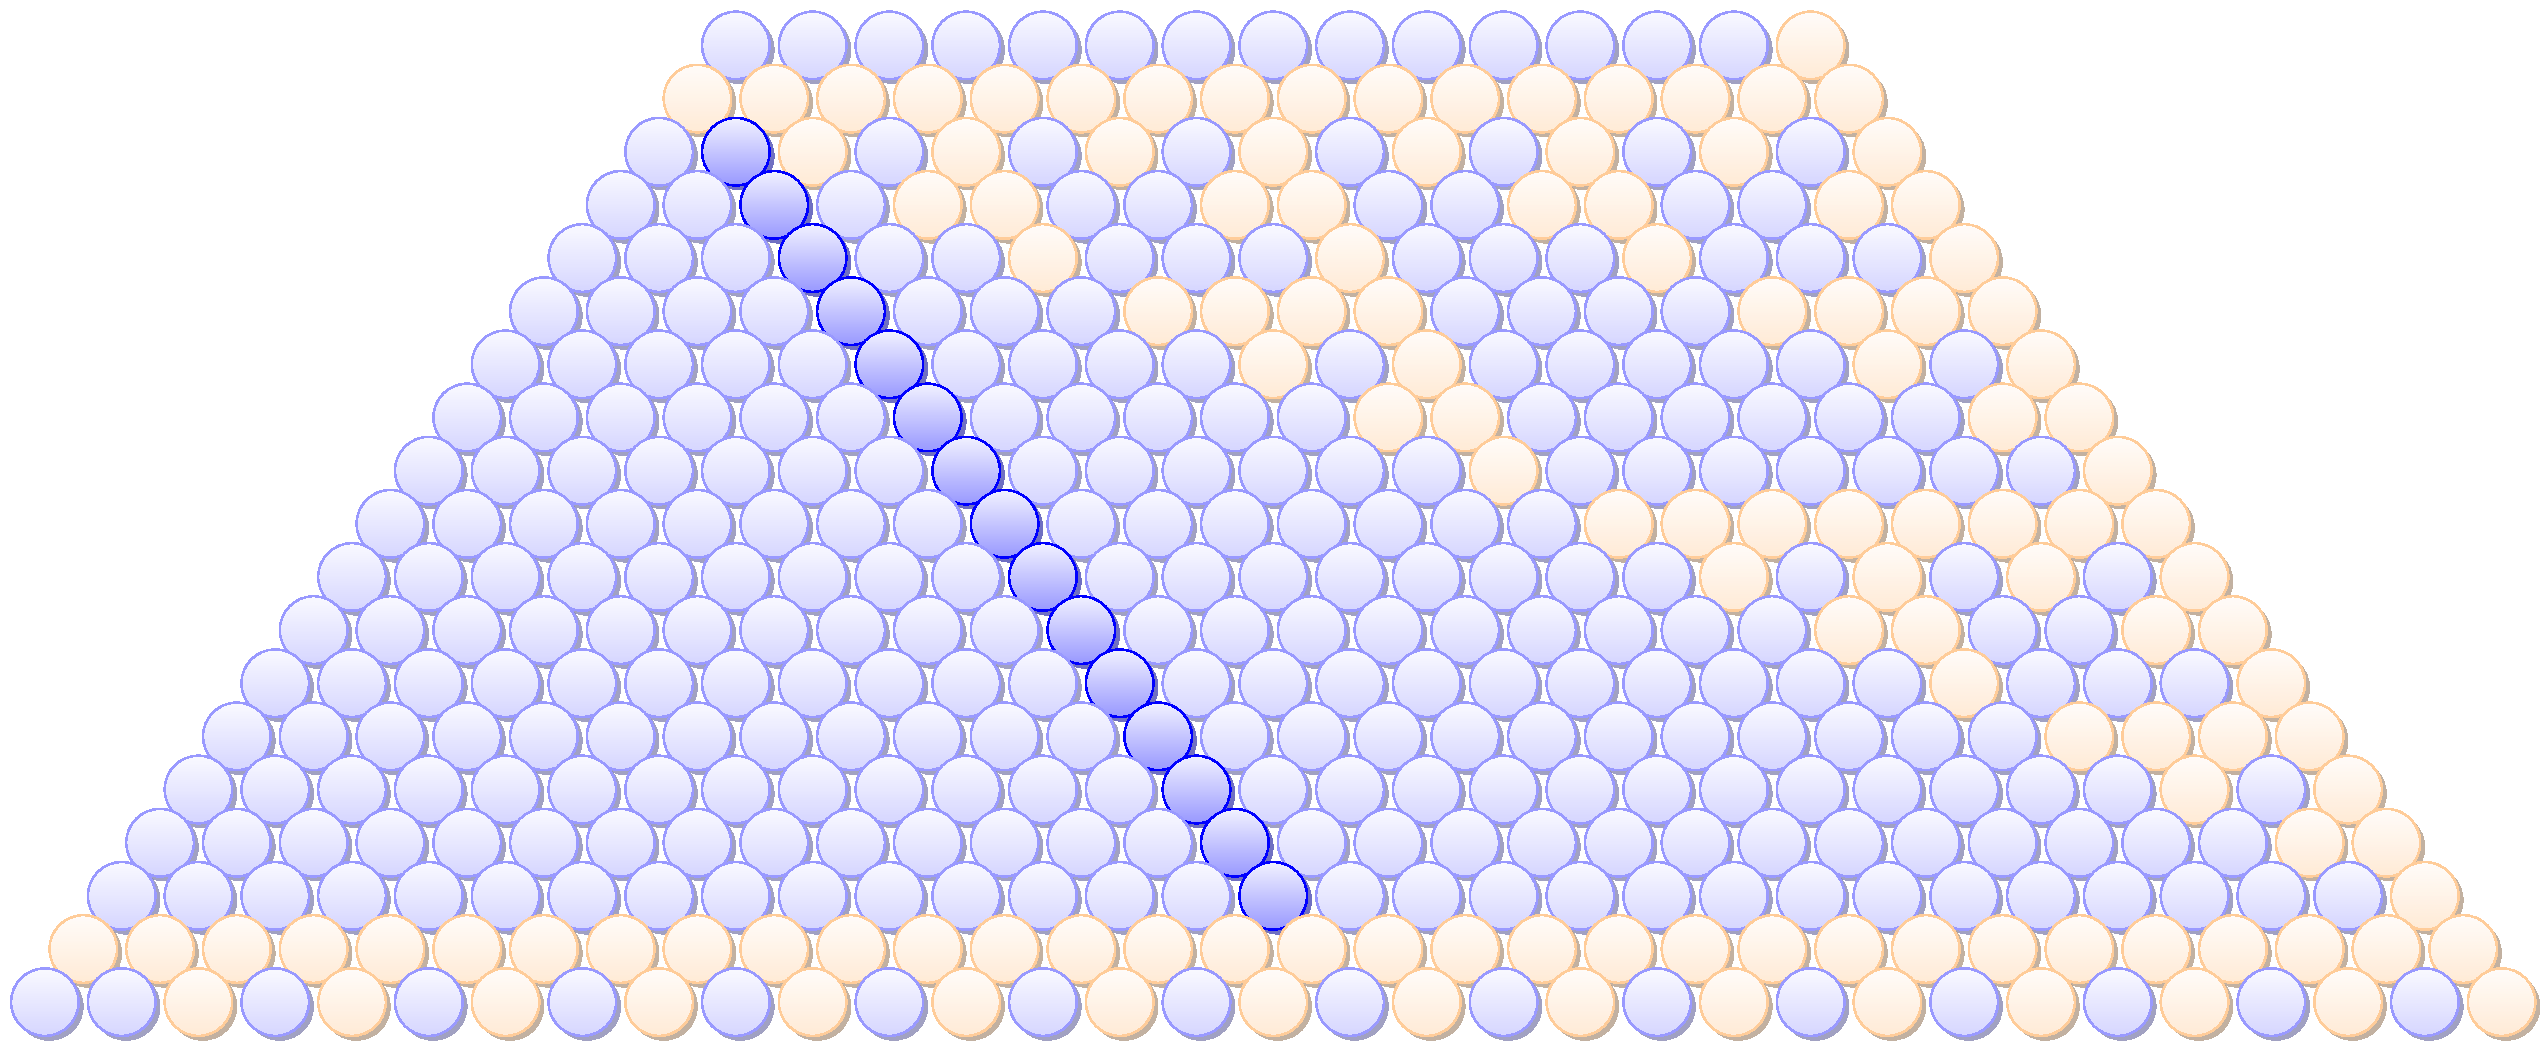
\includegraphics[width=10cm, height=10cm, keepaspectratio=true]{catalan-tikz/mirror-segment/dual-of-mirror-segment.pdf}
    }

    % this 'particular' line is necessary to use `displaymath' environment
    % into the caption environment, togheter with the inclusion of 
    % `caption' package. See here for more explanation:
    % http://stackoverflow.com/questions/2716227/adding-an-equation-or-formula-to-a-figure-caption-in-latex
    \captionsetup{singlelinecheck=off}
    \caption[.]{ segment $S=\lbrace2^{4},\ldots,2^{5}-2\rbrace$ of column $2^{4}-1$,
        $\textcolor{blue}{d_{s,2^{4}-1}}\equiv_{2}0$ for $s\in S$}



    \label{fig:mirror-segment}

\end{figure}
